\documentclass[12pt]{beamer}
\usepackage[spanish]{babel}
\usepackage[utf8]{inputenc}
\usepackage{xcolor}
\usepackage{listings}
\usepackage{palatino}
\usepackage{fancyvrb}
\usepackage{amsmath}
\usepackage{graphics}

\usecolortheme{crane}
\usefonttheme{serif}

\title{Archivos}
\author{
  Roberto Bonvallet \\
  \url{roberto.bonvallet@usm.cl} \\
  \url{http://progra.8o.cl}
}

\lstloadlanguages{fortran}
\lstset{language=fortran,basicstyle=\small,%
        morestring=[b]',stringstyle=\it,showstringspaces=false}
\fvset{formatcom=\small,frame=single,gobble=6,commandchars=\\\{\}}

\begin{document}
  \begin{frame}
    \maketitle
  \end{frame}

  \begin{frame}
    \frametitle{El computador}
    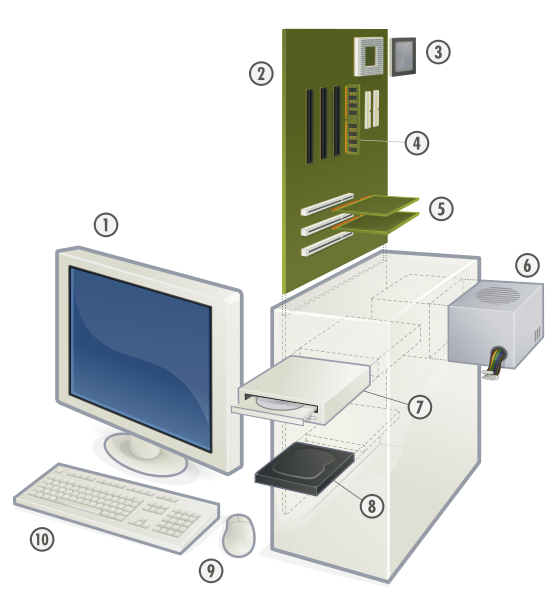
\includegraphics[scale=.4]{compu}
  \end{frame}

  \begin{frame}
    \frametitle{Unidades de almacenamiento}
    \begin{columns}[t]
      \column{0.5\textwidth}
        \begin{itemize}
          \item memoria RAM:
            \begin{itemize}
              \item volátil
              \item acceso directo
              \item rápida {\tiny($\sim$ns)}
              \item cara {\tiny(\$10k/GB)}
              \item poca capacidad {\tiny($\sim$GB)}
              \item contiene variables e instrucciones
            \end{itemize}
        \end{itemize}
      \column{0.5\textwidth}
        \begin{itemize}
          \item disco duro:
            \begin{itemize}
              \item persistente
              \item acceso secuencial
              \item lento {\tiny($\sim$ $\mu$s)}
              \item barato {\tiny(\$100/GB)}
              \item mucha capacidad {\tiny($\sim$TB)}
              \item contiene \alert{archivos}
            \end{itemize}
        \end{itemize}
    \end{columns}
  \end{frame}

  \begin{frame}[fragile]
    \frametitle{Archivos}
    \begin{itemize}
      \item \emph{Unit}: número asociado al archivo
      \item Operaciones:
        \begin{itemize}
          \item abrir un archivo
          \item escribir datos en el archivo
          \item leer datos del archivo
          \item guardar el archivo
        \end{itemize}
        \pause
        \begin{lstlisting}[frame=single,gobble=6]
          open (unit=10, file='archivo.txt', ...)
          write (10, *), a
          read (10, *), b
          close (10)
        \end{lstlisting}
        \pause
      \item Dos tipos de archivo:
        \begin{itemize}
          \item archivo de texto (``un string infinito'')
          \item archivo binario (``un arreglo infinito'')
        \end{itemize}

    \end{itemize}
    
\end{frame}

  \begin{frame}
      \frametitle{Ver ejemplos}
  \end{frame}

  \begin{frame}
      \frametitle{Control 5}
      \pause

      Una canción tiene los siguientes datos: título, artista, álbum,
      duración (en segundos), fecha de grabación (día, mes y año).

      Escriba un programa que permita ingresar los datos de 100 canciones,
      y a continuación
      muestre los títulos de las canciones grabadas en abril. 

      Use registros llamados \texttt{fecha} y \texttt{cancion}.
  \end{frame}

\end{document}
